\subsection{Komplexe Zahlen 1}
\Aufgabe{
    Es gelte für folgende komplexe Zahlen: \\
    $Z_1 = 3+j4$  \\
    $Z_2 = 2-j$   \\
    $Z_3 = j7$    \\
    
    Berechnet werden sollen folgende Aufgabenteile:
    \begin{itemize}
        \item [\bf a)] $Z_1 + Z_2$
        \item [\bf b)] $Z_1 - Z_3$
        \item [\bf c)] Polarform von $Z_1$, $Z_2$ und $Z_3$
        \item [\bf d)] $Z_1 \cdot Z_2$
        \item [\bf e)] $\frac{Z_1}{Z_3}$
        \item [\bf f)] Zeigerdiagramm von $Z_1 + Z_2$ und $Z_1 \cdot Z_2$
    \end{itemize}
}


\Loesung{
    \begin{itemize}

        \item[\bf a)]   $Z_1 + Z_2$\\
              \begin{eqa}
                  Z_1 + Z_2 &= (3 + j4) + (2 - j) \nonumber   \\
                  &= 5 + j3   \nonumber   
              \end{eqa}
              
              
        \item[\bf b)] $Z_1 - Z_3$\\\\
              
              \begin{eqa}
                  Z_1 - Z_3 &= (3 + j4) - (0 + j7)    \nonumber   \\ 
                  &= 3 - j3   \nonumber   
              \end{eqa}
              
        \item[\bf c)] Polarform von $ Z_1, Z_2$ und $Z_3 $\\
              
              \begin{eqa}
                  Z_1 &= 5 \cdot \mathrm{e}^{\mathrm{j}53.13^\circ}  \nonumber  \\
                  Z_2 &= 2,236 \cdot \mathrm{e}^{\mathrm{j}-26,57^\circ}  \nonumber \\
                  Z_3 &= 7 \cdot \mathrm{e}^{\mathrm{j}90^\circ}   \nonumber 
              \end{eqa}
              
              
        \item[\bf d)] $Z_1 \cdot Z_2$\\
              
              \begin{eqa}
                  Z_1 \cdot Z_2 &= (3 + j4) \cdot (2 - j) \nonumber   \\
                  &= 10 + j5  \nonumber
              \end{eqa}
              
              
        \item[\bf e)] $\frac{Z_1}{Z_3} $\\
              
              \begin{eqa}
                  \frac{Z_1}{Z_3} = \frac{3 + j4}{j7} \nonumber
              \end{eqa}
              
              (Erweitern mit dem konjugierten Wert des Nenners, also -j7)\\
              
              \begin{eqa}
                  \frac{3 + j4}{j7} \cdot \frac{-j7}{-j7} = \frac{(3 + j4) \cdot (-j7)}{(j7) \cdot (-j7)}     \nonumber
              \end{eqa}
              
              Hinweis: $j^2 = -1$\\
              
              \begin{eqa}
                  \frac{Z_1}{Z_3} &= \frac{28 - j21}{49} = \frac{28}{49} - j \frac{21}{49} = \frac{4}{7} - j \frac{3}{7}  \nonumber   \\
                  &= \frac{4}{7} - j \frac{3}{7}    \nonumber
              \end{eqa}
              
              
              \newpage
              
        \item[\bf f)] Zeigerdiagramm von $Z_1 + Z_2 $ und $Z_1 \cdot Z_2 $
              
              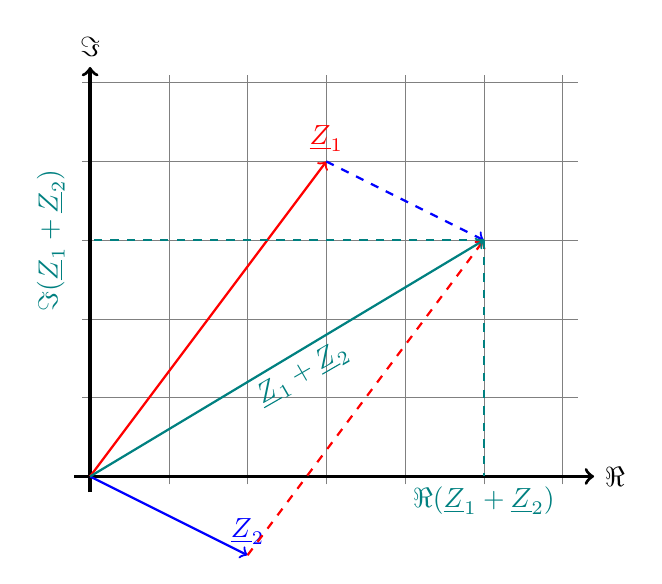
\begin{tikzpicture}
    \draw (0,0) coordinate (K);
    \draw[very thin,gray] (-0.1,-0.1) grid (6.2,5.1);
    \draw[->, very thick] (-0.2,0) -- (6.4,0) node[right] {$\Re$};
    \draw[->, very thick] (0,-0.2) -- (0,5.2) node[above] {$\Im$};
    \draw[->, thick, red] (0,0) -- (3,4) node[above] {$\underline{Z}_\mathrm{1}$};
    \draw[->, thick, blue] (0,0) -- (2,-1) node[above] {$\underline{Z}_\mathrm{2}$};


    \draw[->, dashed, thick, blue] (3,4) -- (5,3) ;
    \draw[->, dashed, thick, red] (2,-1) -- (5,3) ;


    \draw[->, thick, teal] (0,0) -- (5,3);
    \draw(2.7,1.3) node [teal, rotate=30] {$\underline{Z}_\mathrm{1}+\underline{Z}_\mathrm{2}$};
    \draw[dashed, thick, teal] (5,3) -- (0,3)
    (-0.5,3) node[rotate=90] {$\Im(\underline{Z}_\mathrm{1}+\underline{Z}_\mathrm{2}$)};
    \draw[dashed, thick, teal] (5,3) -- (5,0) node[below] {$\Re(\underline{Z}_\mathrm{1}+\underline{Z}_\mathrm{2}$)};
\end{tikzpicture}\\
              %{{\bf Addition von komplexen Zahlen.} Zeichnerische Lösung einer Addition von zwei komplexen Zahlen im Zeigerdiagramm}\\
              
              
              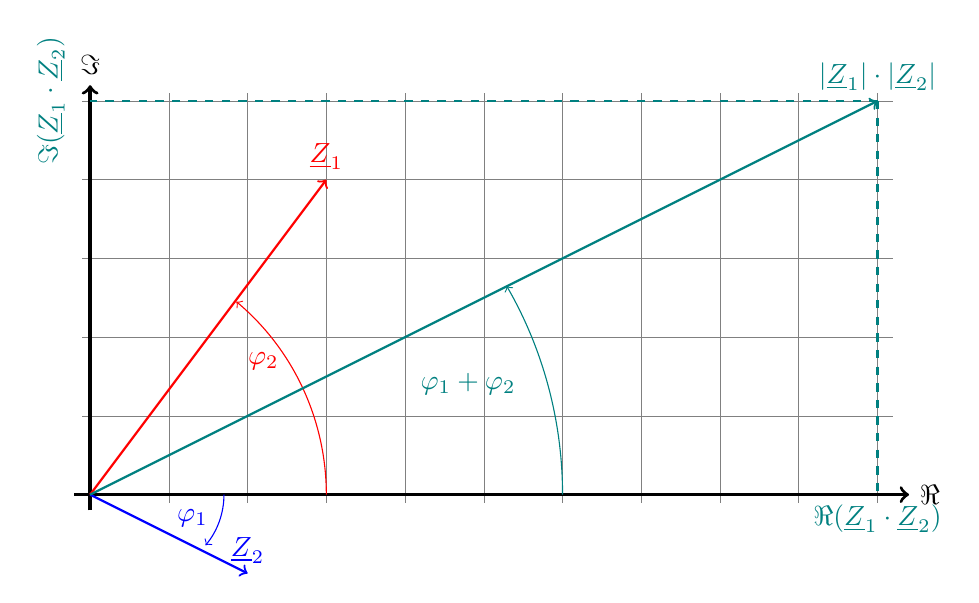
\begin{tikzpicture}
                  \draw (0,0) coordinate (K);
                  \draw[very thin,gray] (-0.1,-0.1) grid (10.2,5.1);
                  \draw[->, very thick] (-0.2,0) -- (10.4,0) node[right] {$\Re$};
                  \draw[->, very thick] (0,-0.2) -- (0,5.2) node[above] {$\Im$};
                  
                  \draw[->, thick, red] (0,0) -- (3,4) node[above] {$\underline{Z}_\mathrm{1}$};
                  \draw[->, thick, blue] (0,0) -- (2,-1) node[above] {$\underline{Z}_\mathrm{2}$};
                  \draw [->,blue] (1.7,0) arc (0:-40:1cm);
                  \draw [->,red] (3,0) arc (0:50:3.2cm);
                  \draw [->,teal] (6,0) arc (0:30:5.3cm);
                  \draw[->, thick, teal] (0,0) -- (10,5) node [above] {$|\underline{Z}_\mathrm{1}| \cdot |\underline{Z}_\mathrm{2}|$};
                  % {{\bf Multiplikation von komplexen Zahlen.} Zeichnerische Lösung einer Multiplikation von zwei komplexen Zahlen im Zeigerdiagramm}
                  \draw[dashed, thick, teal] (10,5) -- (10,0) node[below] {$\Re(\underline{Z}_\mathrm{1} \cdot \underline{Z}_\mathrm{2}$)};
                  \draw[dashed, thick, teal] (10,5) -- (0,5)
                  (-0.5,5) node[rotate=90] {$\Im(\underline{Z}_\mathrm{1} \cdot \underline{Z}_\mathrm{2}$)};
                  \node [red] at (2.2,1.7) {$\varphi_\mathrm{2}$};
                  \node [blue] at (1.3,-0.3) {$\varphi_\mathrm{1}$};
                  
                  \node [teal] at (4.8,1.4) {$\varphi_\mathrm{1} + \varphi_\mathrm{2}$};
              \end{tikzpicture}\\
              
              
              
    \end{itemize}
    
}